\section{Circuits}
\subsection*{Switch with Transients 1}
It's been a long time. All transients have died out.
\begin{center}
  \begin{circuitikz}[
    american, scale = 0.6, transform shape
  ]
    \ctikzset{
      batteries/scale=0.7,
      resistors/scale=0.55,
      capacitors/scale=0.6,
      bipoles/cuteswitch/thickness=0.3
      % font=\footnotesize
    }
    \draw
      (0,0) to[battery, l_=$\qty{28}{\volt}$] ++(0,2)
      to[R, l=$\qty{4}{\kilo\ohm}$] ++(2,0)
      % to[short] ++(1,0)
      to[cute opening switch, invert, name=swlbl] ++(1,0) coordinate(swtch)
      to[cute inductor,l^=$\qty{200}{\milli\henry}$] ++(0,-2) coordinate(lpbck1)
      -- (0,0)
    ;
    \draw[draw=black, dash pattern=on 1pt off 1pt]
      (swlbl.in) to[short] ++(0,0.75) coordinate(swdash)
    ;
    \draw
      (swdash) to[short, o-] ++(0,0.5)
      to[R, l=$\qty{24}{\kilo\ohm}$] ++(2,0)
      to[short, -*] ++(0,-1.25)
      to[curved capacitor,l=$\qty{8}{\nano\farad}$] ++(2,0)
      to[battery, l=$\qty{20}{\volt}$] ++(0,-2)
      to[short, -*] (lpbck1)
      (swlbl.in) to[R, l=$\qty{12}{\kilo\ohm}$] ++(2,0)
    ;
    \node[below] at (swlbl.out){a};
    \node[left] at (swdash){b};
  \end{circuitikz}
\end{center}
At $t=0^-$ for the capacitor current thru is 0 and voltage across is
\qty{20}{\volt} (higher to the right). For the inductor current thru is
\qty{7}{mA} (updward) and voltage across is 0.

At $t=0^+$ for the capacitor current thru is \qty{7}{mA} (left-to-right)
and voltage across is preserved. For the inductor current thru is
preserved and voltage across is \qty{56}{\volt} (higher at the top)
given by\\
\begin{scriptsize}
  $V_C(0^+) + \qty{20}{\volt} - V_L(0^+) + \qty{8}{\kilo\ohm}(\qty{7}{\milli\ampere})=0.$
\end{scriptsize}\\
The capacitor voltage at $0^+$ is \qty{20}{\volt} which is negative for
a CW KVL, so only the last term remains and we get \qty{56}{\volt}.

\subsection*{Second Order Circuit}
\begin{center}
  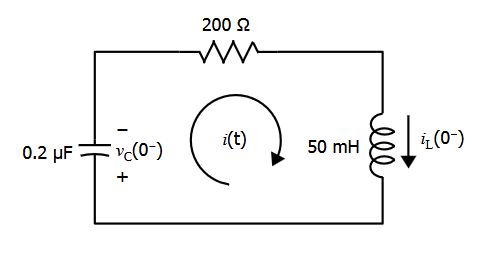
\includegraphics[scale=0.4]{second-order-final-pp.png}
\end{center}
This is a second-order circuit. There is an initial voltage on the
capacitor (assuming clockwise current) $v(0^-)=+\qty{12}{\volt}$, and an
initial current in the inductor $i_L(0^-)=\qty{30}{\milli\ampere}$
clockwise. In order to solve the differential equation for $i(t)$, the
initial voltages $v_L(0^+)$ and $v_R(0^+)$, and
$\left.\frac{d}{dt}i(t)\right\vert_{t=0^+}$ must be found. Using what
you know about inductors, capacitors, and KCL, find these values.\\
\begin{scriptsize}
  $i\left(0^+\right)=i_L\left(0^-\right)=\qty{30}{\milli\ampere}$\\
  $v_C\left(0^+\right)=v_C\left(0^-\right)=\qty{12}{\volt}$\\
  $v_R\left(0^+\right)=i\left(0^+\right)R=\qty{6}{\volt},~\text{+ to left}$\\
  $\text{KVL at }t=0^+:~+6+12+v_L\left(0^+\right)=0$\\
  $v_L\left(0^+\right)=\qty{-18}{\volt},~\text{+ at bottom}$\\
  since $v_L\left(0^+\right)=L\left.\frac{d}{dt}i\left(t\right)\right\vert_{t=0^+}$\\
  $\left.\frac{d}{dt}i\left(t\right)\right\vert_{t=0^+}=\frac{v_L\left(0^+\right)}{L}=-\qty{360}{\ampere\per\second}$\\
\end{scriptsize}

\subsection*{Max Power Transfer}
\begin{center}
  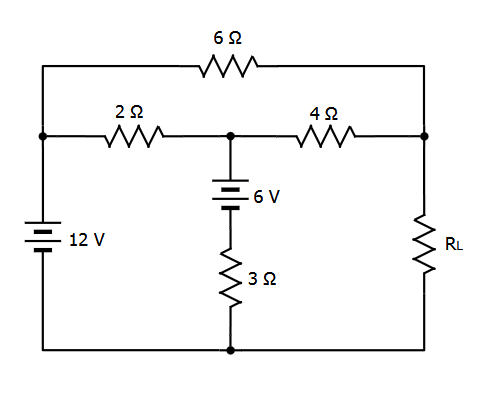
\includegraphics[scale=0.4]{max-power-final-pp.png}
\end{center}
Find the value of $R_L$ for maximum power transfer to $R_L$. First, Find
Thevenin Equiv Resistance.

Setup system for open circuit voltage (assume $R_L$ is not there)\\
\begin{scriptsize}
  $V_{1}=12$\\
  $\frac{V_{2}-12}{2}+\frac{V_{2}-6}{3}+\frac{V_{2}-V_{OC}}{4}=0$\\
  $\frac{V_{OC}-V_{2}}{4}+\frac{V_{OC}-12}{6}=0$\\
\end{scriptsize}
Solve system\\
\begin{scriptsize}
  $V_{2}\approx\qty{9.8571}{\volt}$\\
  $V_{OC}\approx\qty{10.7143}{\volt}$\\
\end{scriptsize}
Setup system for short circuit current (assume $R_L$ is a short). $V_3$
is the same node that $V_2$ were\\
\begin{scriptsize}
  $\frac{V_{3}-12}{2}+\frac{V_{3}-6}{3}+\frac{V_{3}}{4}=0$\\
\end{scriptsize}
Solve system\\
$V_{3}=\qty{7.3846}{\volt}$\\
Now compute currents thru \qty{6}{\ohm} and \qty{4}{\ohm} resistors\\
\begin{scriptsize}
  $I_{4}=\frac{V_{1}}{4}=\qty{1.8462}{\ampere}$\\
  $I_{6}=\frac{12}{6}   =\qty{2}{\ampere}$\\
\end{scriptsize}
By KCL\\
$I_{SC}=I_{4}+I_{6}=\qty{3.8462}{\ampere}$\\
Finally\\
$R_{L}=R_{th}=\frac{V_{OC}}{I_{SC}}=\qty{2.79}{\ohm}$

\subsection*{Output Impedance 1}
\begin{center}
  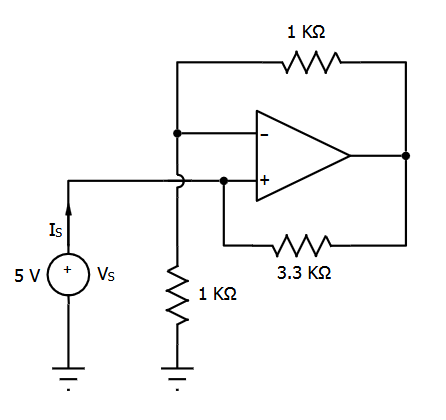
\includegraphics[scale=0.4]{op-amp-final-pp.png}
\end{center}
Setup system from nodes\\
\begin{scriptsize}
  $\frac{v_n}{\qty{1}{\kilo\ohm}} + \frac{v_n-v_{oa}}{\qty{1}{\kilo\ohm}} = 0$\\
  $\frac{v_p - v_{oa}}{\qty{3.3}{\kilo\ohm}} - I_S = 0$\\
\end{scriptsize}
Solve system\\
$v_{oa} = \qty{10}{\volt};~~I_S\approx\qty{-1.515}{\milli\ampere}$\\
Finally\\
$R_{in} \approx \frac{\qty{5}{\volt}}{\qty{-1.515}{\milli\ampere}} = \qty{-3.3}{\kilo\ohm}$

\subsection*{Dependent Sources}
\begin{center}
  \begin{circuitikz}[american, scale = 0.625, transform shape]
    \ctikzset{
      inductors/scale=1,
      sources/scale=0.75,
      csources/scale=0.75,
      resistors/scale=0.625,
      capacitors/scale=0.625
    }
    % x: 7 divs (1 unit each), y: 2.5 divs (1 unit each)
    \draw
      (1,2.5) to[R=$\qty{10}{\ohm}$, *-] ++(0,-1.5) % res 10 ohm
      to[short, -*] ++(0,-1) % res 10 ohm
      to[short] ++(-1,0) % short
      to[isource, l_=$10.6\Angle\qty{0}{\degree}\unit{\ampere}$] ++(0,1.5) % curr src 10.6 ang 0 deg
      to[short] ++(0,1) % short
      to[short] ++(1,0) % short
      to[R=$\qty{1}{\ohm}$] ++(2,0) % res 1 ohm
      to[cute inductor,i>_=$i_x$,l^=$j\qty{2}{\ohm}$] ++(2,0) % indc j2 ohm
      to[curved capacitor,l_=$-j\qty{5}{\ohm}$, *-*] ++(0,-2.5) % cap -j5 ohm
      to[short] ++(2,0) % short
      to[cV,l=$\qty{20}{\ohm}i_x$, invert] ++(0,2.5) % dep volt src 20 * i_x
      to[R=$\qty{5}{\ohm}$] ++(-2,0) % res 5 ohm
      (1,0) to[short] ++(4,0) % short
    ;
    \node[above] at (1,2.5){$v_1$};
    \node[above] at (5,2.5){$v_2$};
  \end{circuitikz}
\end{center}
First simplify series impedance\\
$\Rightarrow\qty{1}{\ohm}+j\qty{2}{\ohm} = \acimp{\sqrt{5}}{\arctan(2)}$\\
Then set KCL\\
\begin{scriptsize}
  $\text{node at }v_1 : \acamp{-10.6}{0} + \frac{v_1}{\qty{10}{\ohm}} + i_x = \qty{0}{\ampere}$ \\
  $\text{node at }v_2 : -i_x + \frac{v_2}{-\acimp{5}{90}} + \frac{v_2-\qty{20}{\ohm}i_x}{\qty{5}{\ohm}} = \qty{0}{\ampere}$\\
\end{scriptsize}
also\\
$i_x = \frac{v_1-v_2}{\acimp{\sqrt{5}}{\arctan(2)}}$\\
Solve system.

\subsection*{Op Amp Example 1}
\begin{center}
  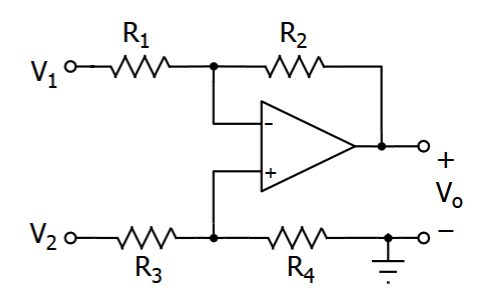
\includegraphics[scale=0.4]{op-amp-simpl-1.png}
\end{center}
Assume that $R_1=R_3$ and $R_2=R_4$, then\\
$V_O=\frac{R_2}{R_1}\left(V_2-V_1\right)$
\subsection*{Switched Capacitor}
\begin{center}
  \begin{circuitikz}[american, scale = 0.6, transform shape]
    \ctikzset{bipoles/cuteswitch/thickness=0.3}
    \draw
    (0,0) to[battery, l=5V, invert] (0,3) % Battery
    to[cute closing switch, name=Sw] (3,3) % Switch
    to[R=$\qty{10}{\ohm}$] (6,3) % Resistor
    to[curved capacitor,l=$\qty{1}{\micro\farad}$, name=Cap] (6,0) % Capacitor with voltage label
    -- (0,0); % Ground connection
    \node[below] at (Sw){$t=0$};
    \node[left=0.5cm] at (Cap){$v_C(0^-)=\qty{2}{\volt}$};
  \end{circuitikz}
\end{center}
Equation is $v_C(t) = V_s + Ke^{-\frac{t}{RC}}$\\
in case you need it diff. eqn. is\\
$\frac{d}{dt}v_C(t)+\frac{v_C(t)}{RC} = \frac{V_s}{RC}$ \\
Plug and chug you get $K = \boxed{\qty{-3}{\volt}}$. And in equation
form\\
$v_C(t) = \boxed{\qty{5}{\volt} + (\qty{-3}{\volt})e^{-\frac{t}{\qty{10}{\micro\second}}}}$

\subsection*{Op Amp with Cap}
\begin{center}
  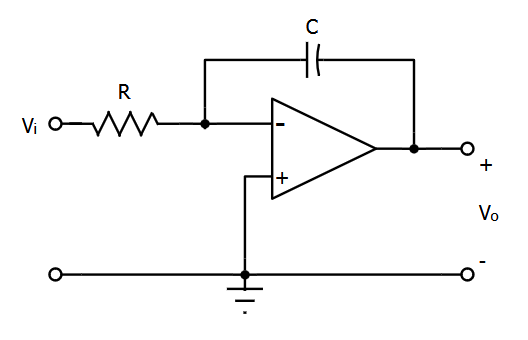
\includegraphics[scale=0.35]{op-amp-vcr.png}
\end{center}
Find $V_o$ as a function of $V$, $C$, and $R$.\\
$\frac{0-V_i}{R}+C\frac{d}{dt}\left(0-V_o\right)=0$\\
$\frac{d}{dt}V_o=-\left(\frac{1}{RC}\right)V_i$\\
$V_o=-\left(\frac{1}{RC}\right)\int V_idt$
